\documentclass[aspectratio=169,9pt]{beamer}
\usetheme[progressbar=frametitle,numbering=fraction]{metropolis}
\usepackage[utf8]{inputenc}
\usepackage[T1]{fontenc}
\usepackage{amsmath,amssymb}
\usepackage{graphicx}
\usepackage{booktabs}
\usepackage{tabularx}
\usepackage{siunitx}
\usepackage{tikz}
\usetikzlibrary{arrows.meta,positioning,calc}
\usepackage{listings}
\sisetup{detect-all}
\definecolor{cBlue}{HTML}{2A6FBB}
\definecolor{cGreen}{HTML}{2A9D55}
\definecolor{cOrange}{HTML}{E07B39}
\definecolor{cGrey}{HTML}{6B7280}
\definecolor{codebg}{HTML}{F3F4F6}
\newcommand{\um}{\,\si{\micro\metre}}
\lstset{basicstyle=\ttfamily\scriptsize,backgroundcolor=\color{codebg},frame=none,columns=fullflexible,keepspaces=true,
  showstringspaces=false,commentstyle=\color{cGrey},breaklines=true,xleftmargin=2pt,aboveskip=3pt,belowskip=3pt}
\tikzset{box/.style={draw,rounded corners=2pt,align=center,font=\scriptsize,minimum height=11mm,text width=27mm,fill=#1!10,draw=#1!70},box/.default=cBlue}

\title{How to use the AFM force-volume pipeline}
\subtitle{Installation, input data structure, configuration file, the four steps, outputs, troubleshooting}
\date{\texttt{afm\_ting\_pipeline.py} $\cdot$ \texttt{extract\_topo\_E.py} $\cdot$ \texttt{segment\_cells.py} $\cdot$ \texttt{build\_timelapse\_viewer.py} $\cdot$ \texttt{afm\_pipeline.toml}}
\author{}

\begin{document}
\maketitle

\begin{frame}{Overview: four scripts, one parameter file}
\centering
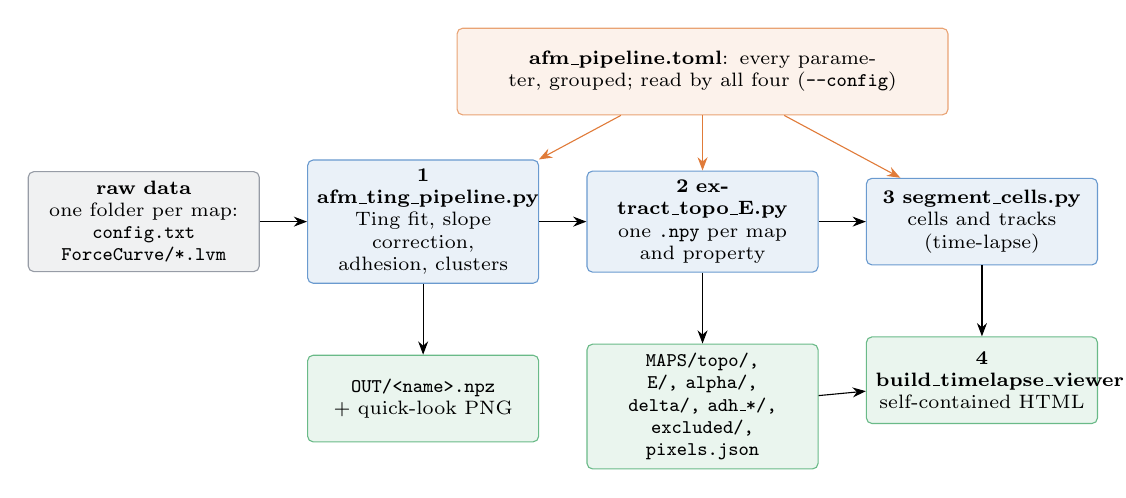
\begin{tikzpicture}[node distance=5mm and 6mm,>=Stealth]
\node[box=cGrey] (raw) {\textbf{raw data}\\one folder per map:\\\texttt{config.txt}\\\texttt{ForceCurve/*.lvm}};
\node[box,right=of raw] (s1) {\textbf{1 afm\_ting\_pipeline.py}\\Ting fit, slope correction,\\adhesion, clusters};
\node[box,right=of s1] (s2) {\textbf{2 extract\_topo\_E.py}\\one \texttt{.npy} per map\\and property};
\node[box,right=of s2] (s3) {\textbf{3 segment\_cells.py}\\cells and tracks\\(time-lapse)};
\node[box=cGreen,below=9mm of s3] (s4) {\textbf{4 build\_timelapse\_viewer.py}\\self-contained HTML};
\node[box=cGreen,below=9mm of s1] (npz) {\texttt{OUT/<name>.npz}\\+ quick-look PNG};
\node[box=cGreen,below=9mm of s2] (maps) {\texttt{MAPS/topo/, E/, alpha/,}\\\texttt{delta/, adh\_*/, excluded/,}\\\texttt{pixels.json}};
\draw[->] (raw)--(s1); \draw[->] (s1)--(s2); \draw[->] (s2)--(s3);
\draw[->] (s1)--(npz); \draw[->] (s2)--(maps); \draw[->] (s3)--(s4); \draw[->] (maps)--(s4);
\node[box=cOrange,above=7mm of s2,text width=60mm] (cfg) {\textbf{afm\_pipeline.toml}: every parameter, grouped; read by all four (\texttt{--config})};
\draw[->,cOrange] (cfg) -- (s1); \draw[->,cOrange] (cfg) -- (s2); \draw[->,cOrange] (cfg) -- (s3);
\end{tikzpicture}\\[4pt]
\small Steps 1--2 are enough for single maps. Steps 3--4 are for time-lapses (several maps of the same specimen). The viewer also works without step 3.
\end{frame}

% ===========================================================================
\section{Installation}

\begin{frame}[fragile]{Installation (macOS, Linux, Windows)}
\small
\textbf{Requirements}:
\begin{itemize}
\item Python $\ge$ 3.9; numpy ($\ge$ 1.20), scipy ($\ge$ 1.6), scikit-image ($\ge$ 0.19, for segmentation), matplotlib (quick-look images).
\item Python $\ge$ 3.11 reads the config file natively. Older versions use \texttt{tomli} if it is installed, otherwise a built-in reader.
\end{itemize}
\begin{lstlisting}
# macOS / Linux (Terminal)
python3 -m venv afm-env && source afm-env/bin/activate
pip install numpy scipy scikit-image matplotlib

# Windows (PowerShell)
py -m venv afm-env ; .\afm-env\Scripts\Activate.ps1
pip install numpy scipy scikit-image matplotlib
\end{lstlisting}
\textbf{Files}: put the four scripts and \texttt{afm\_pipeline.toml} in one folder. \texttt{segment\_cells.py} imports \texttt{build\_timelapse\_viewer.py} from the same folder.\\[3pt]
\textbf{CPU}: every script uses 80\,\% of the cores by default (\texttt{[run] cores}: a fraction $\le1$, or a number of workers $>1$). On Windows at most 61 workers.\\[3pt]
\textbf{Help}: \texttt{python <script>.py -h} lists all options.
\end{frame}

% ===========================================================================
\section{Input data}

\begin{frame}[fragile]{Input data structure}
\begin{columns}[T]
\begin{column}{0.47\textwidth}
\begin{lstlisting}
data_20260515_0.25nN/          <- any root
  sample_ciona/
    data_171551/               <- one map
      config.txt
      ForceCurve/
        ForceCurve_00000.lvm
        ForceCurve_00001.lvm
        ...
        ForceCurve_02774.lvm
    data_172222/
      config.txt
      ForceCurve/...
    ...
    data_214803/
\end{lstlisting}
\end{column}
\begin{column}{0.51\textwidth}\small
\begin{itemize}
\item \textbf{A data set} = any folder that contains \texttt{config.txt} and \texttt{ForceCurve\_<number>.lvm} files, either in a \texttt{ForceCurve/} sub-folder or directly in the folder.
\item Files are sorted by the \textbf{number} in the name, which is the acquisition order. Missing files become empty pixels (with a warning).
\item \textbf{Output name} = the last 3 path components joined by \_ (\texttt{[run] name\_depth}), e.g.\\ \texttt{data\_20260515\_0.25nN\_sample\_ciona\_data\_171551}
\item \textbf{Time-lapse}: the name must \textbf{end in HHMMSS}, the start time of the map. This orders the frames and gives the time axis; runs past midnight are handled.
\end{itemize}
\end{column}
\end{columns}
\end{frame}

\begin{frame}[fragile]{\texttt{config.txt} (written by the instrument) and the \texttt{.lvm} files}
\begin{columns}[T]
\begin{column}{0.36\textwidth}
\begin{lstlisting}
start_time,213626.88
Vtrig,0.060000
Zig,FALSE
num_app,3000
num_ret,3500
xlength,1.500000
ylength,1.500000
Xstep,37
Ystep,75
loop_time,9.000000
...
\end{lstlisting}
\scriptsize Format: \texttt{key,value} per line. Other keys are ignored but kept in the \texttt{.npz}.
\end{column}
\begin{column}{0.62\textwidth}\small
\textbf{Keys used}:
\begin{itemize}
\item \texttt{num\_app}, \texttt{num\_ret}: samples per approach / retract;
\item \texttt{Xstep}, \texttt{Ystep}: pixels per line, number of lines;
\item \texttt{xlength}, \texttt{ylength}: scan size in V. Size $=\text{V}\times$ \texttt{xy\_sensitivity\_um\_per\_V}, so here $1.5\times25=\SI{37.5}{\micro\metre}$ and the pixel is $37.5/37\times37.5/75=1.014\times\SI{0.5}{\micro\metre}$;
\item \texttt{loop\_time}: sample interval in \si{\micro\second};
\item \texttt{Zig}: TRUE if every 2nd line is scanned backwards.
\end{itemize}
\textbf{\texttt{.lvm} file}: one number per line (text), in volts:
\[\underbrace{d_\text{app}}_{\texttt{num\_app}}\ \Big|\ \underbrace{d_\text{ret}}_{\texttt{num\_ret}}\ \Big|\ \underbrace{Z_\text{app}}_{\texttt{num\_app}}\ \Big|\ \underbrace{Z_\text{ret}}_{\texttt{num\_ret}}\]
Pixel order: $x$ fast (along a line), $y$ slow; file 0 is the first point of the first line.
\end{column}
\end{columns}
\end{frame}

% ===========================================================================
\section{The configuration file}

\begin{frame}[fragile]{\texttt{afm\_pipeline.toml}: structure}
\begin{columns}[T]
\begin{column}{0.48\textwidth}
\begin{lstlisting}
[afm]          # 1. NOT in config.txt
invols_nm_per_V         = 200.0
spring_constant_N_m     = 0.09
z_sensitivity_um_per_V  = 25.0
xy_sensitivity_um_per_V = 25.0

[probe]        # 2.
geometry   = "sphere"
radius_um  = 3.0
poisson_ratio = 0.5

[acquisition]  # 3. from config.txt
sample_interval_s = "auto"
zigzag            = "auto"
...                # sections 4-14
\end{lstlisting}
\end{column}
\begin{column}{0.5\textwidth}\footnotesize
Sections in processing order:
\begin{enumerate}\setlength\itemsep{0pt}
\item \texttt{afm}: calibration that is not in \texttt{config.txt}
\item \texttt{probe}: contact model
\item \texttt{acquisition}: overrides of \texttt{config.txt}
\item \texttt{preprocessing}: raw signal $\to$ force
\item \texttt{fit}: Ting fit
\item \texttt{quality}: valid pixels
\item \texttt{clustering}, \texttt{adhesion}
\item \texttt{export}: maps (step 2)
\item \texttt{registration}, \texttt{segmentation}, \texttt{tracking}
\item \texttt{viewer}, \texttt{run}
\end{enumerate}
\textbf{Rules}:
\begin{itemize}
\item The unit is part of every key name.
\item \texttt{"auto"} means the value is derived from the data.
\item Priority: command line $>$ config file $>$ built-in default.
\item Unknown keys are reported (typo check).
\end{itemize}
\end{column}
\end{columns}
\end{frame}

\begin{frame}{Which parameters can be derived from the data?}
\scriptsize
\begin{tabularx}{\textwidth}{@{}l l X@{}}
\toprule
parameter & how it is set & rule\\
\midrule
\multicolumn{3}{@{}l}{\textbf{must be given} (not in the data)}\\
InvOLS, spring constant, $Z$/$XY$ sensitivity & \texttt{[afm]} & calibration of the instrument and cantilever\\
probe geometry and radius, Poisson ratio & \texttt{[probe]} & probe and sample\\
cell diameter $D$ & \texttt{[segmentation]} & biology. A spectral estimate from the maps was not reliable (2--9\um{} across frames)\\
\midrule
\multicolumn{3}{@{}l}{\textbf{read from the data}}\\
sample interval, zig-zag, grid, scan size & \texttt{config.txt} & \texttt{loop\_time}, \texttt{Zig}, \texttt{Xstep/Ystep}, \texttt{xlength/ylength}\\
pixel size of each map (steps 3--4) & \texttt{pixels.json} & written by step 2 from the \texttt{.npz}\\
speeds, drag, noise & computed & from $Z(t)$ and the baselines of every curve\\
\midrule
\multicolumn{3}{@{}l}{\textbf{derived from the data scale} (\texttt{"auto"})}\\
\texttt{block\_average} & samples per curve & $\approx800$ points per curve\\
\texttt{baseline\_samples} & approach length & $\min(600,\ \texttt{num\_app}/3)$\\
\texttt{slope\_smooth\_um} & pixel size, $R$ & $\max(p_x,p_y,R/3)$\\
\texttt{shift\_max\_um} (registration) & field of view & $0.65\times$ FOV\\
segmentation grid, ridge, smoothing, min.\ area & $D$, pixel size & $\min(D/16,p/2)$; $0.08D$, $0.18D$; $0.09D$; $0.15D^2$\\
\texttt{max\_step\_um}, \texttt{refine\_shift\_um} & $D$ & $0.75D$\\
\texttt{display\_grid\_um} (viewer) & pixel size & $\min(p_x,p_y)/2$\\
\midrule
\multicolumn{3}{@{}l}{\textbf{dimensionless} (robust units, ratios, $R^2$): transfer between data sets as they are}\\
\bottomrule
\end{tabularx}
\end{frame}

\begin{frame}[fragile]{Using the config file}
\small
\begin{lstlisting}
# all scripts take the same file; anything on the command line overrides it
python afm_ting_pipeline.py RAW -o OUT --config afm_pipeline.toml
python afm_ting_pipeline.py RAW -o OUT --config afm_pipeline.toml --radius 2.5 --cores 6
\end{lstlisting}
\begin{itemize}
\item Keep one config file per experiment (probe, cantilever) next to the results. Every \texttt{.npz} also stores the parameters actually used (\texttt{params\_json}), including the ``auto'' values.
\item To change only one thing for a test run, use the command line instead of editing the file.
\item A few examples of command-line names: \texttt{--invols}, \texttt{--k}, \texttt{--radius}, \texttt{--geometry}, \texttt{--block}, \texttt{--t0}, \texttt{--r2-min} (step 1); \texttt{--cell-diam}, \texttt{--depth}, \texttt{--channels} (step 3); \texttt{--grid} (step 4).
\end{itemize}
\textbf{Before the first run with a new cantilever or probe}, check:
\begin{itemize}
\item \texttt{invols\_nm\_per\_V} and \texttt{spring\_constant\_N\_m}: $F$ and $E$ scale with both;
\item \texttt{radius\_um}: $E\propto R^{-1/2}$ (Hertz-like);
\item \texttt{xy\_sensitivity\_um\_per\_V}: the pixel size, hence slopes, areas and the registration.
\end{itemize}
\end{frame}

% ===========================================================================
\section{Running the four steps}

\begin{frame}[fragile]{Step 1: fit all force curves}
\begin{lstlisting}
# all data sets below RAW_ROOT
python afm_ting_pipeline.py RAW_ROOT -o results --config afm_pipeline.toml
# selected folders, or a text file with one path per line
python afm_ting_pipeline.py RAW/data_171551 RAW/data_172222 -o results --config afm_pipeline.toml
python afm_ting_pipeline.py datasets.txt -o results --config afm_pipeline.toml
\end{lstlisting}
\begin{columns}[T]
\begin{column}{0.48\textwidth}\small
\begin{itemize}
\item Per data set: load (parallel), drag, vertical Ting fit, slope, normal-frame refit, clusters, adhesion $\to$ \texttt{results/<name>.npz} and \texttt{<name>.png}.
\item Existing results are skipped; use \texttt{--overwrite} to redo them.
\item Time: $\approx\SI{0.3}{\second}$ per curve and core for both fits, plus loading. 2775 curves on 8 cores take $\approx2$ min.
\item The log prints the speeds, drag, valid fraction and medians of $E_1$, $E(t_\text{ref})$, $\alpha$ and adhesion. Check them.
\end{itemize}
\end{column}
\begin{column}{0.5\textwidth}
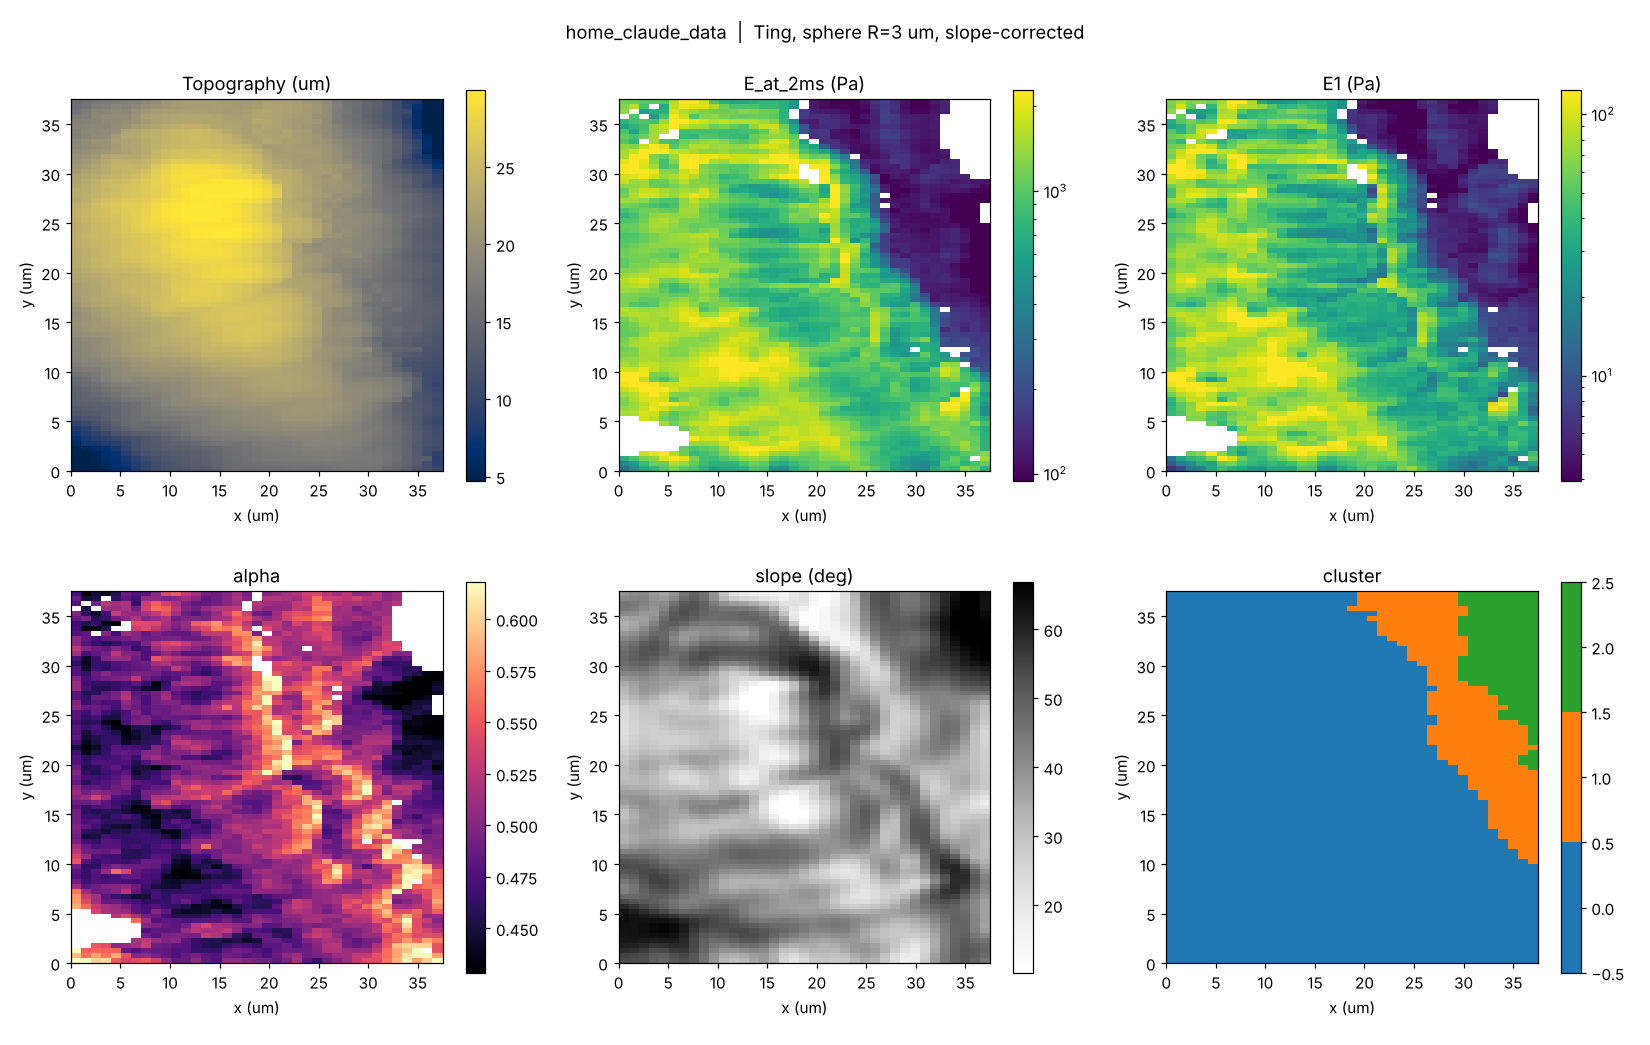
\includegraphics[width=\textwidth]{fig/quicklook.png}\\
\scriptsize Quick-look PNG: height, $E$, $E_1$, $\alpha$, slope, clusters.
\end{column}
\end{columns}
\end{frame}

\begin{frame}[fragile]{Step 2: export maps}
\begin{lstlisting}
python extract_topo_E.py results -o maps --config afm_pipeline.toml
\end{lstlisting}
\begin{columns}[T]
\begin{column}{0.4\textwidth}
\begin{lstlisting}
maps/
  topo/<name>.npy      height (um)
  E/<name>.npy         E (Pa), [export] e_map
  alpha/<name>.npy
  delta/<name>.npy     max. indentation (um)
  adh_force_nN/ ... adh_tether_len_um/
  excluded/<name>.npy  bitmask (0 = valid)
  pixels.json          pixel size per map
\end{lstlisting}
\end{column}
\begin{column}{0.58\textwidth}\small
\begin{itemize}
\item Every \texttt{.npy} is a 2D array of shape (lines $\times$ points per line). Row 0 is the first scan line; zig-zag is already undone.
\item \texttt{no\_mask = true} keeps all fitted values. \texttt{excluded} says why a pixel failed: 1 $R^2$, 2 slope, 4 depth, 8 bound, 16 no fit.
\item \texttt{e\_map}: \texttt{E1\_Pa}, \texttt{E\_at\_2ms\_Pa}, \texttt{E\_at\_10ms\_Pa} or \texttt{E1\_vertical\_Pa}. For stiffness comparisons, $E$ at ms is more robust than $E_1$ (see the Ting presentation).
\item \texttt{recompute\_adhesion = true} recomputes the adhesion maps from the stored curves with new \texttt{[adhesion]} parameters, without refitting.
\item The quality thresholds can be changed here without refitting.
\end{itemize}
\end{column}
\end{columns}
\end{frame}

\begin{frame}[fragile]{Step 3: cell segmentation and tracking (time-lapse)}
\begin{lstlisting}
python segment_cells.py maps -o seg --config afm_pipeline.toml   # uses [segmentation] cell_diameter_um
\end{lstlisting}
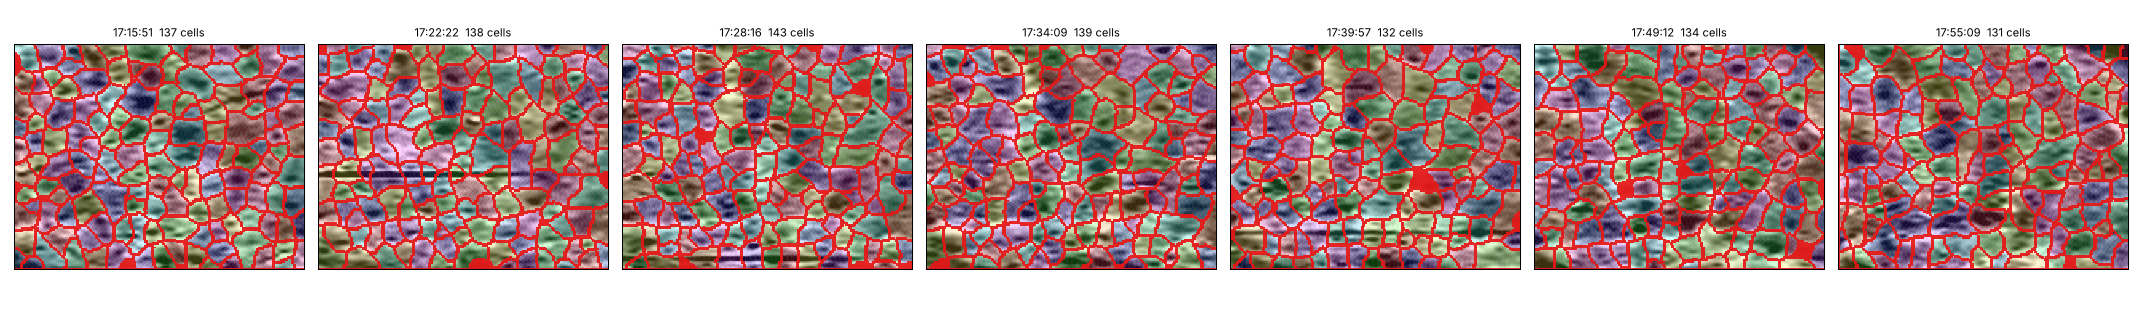
\includegraphics[width=\textwidth]{fig/seg_overview_row.png}
\small
\begin{columns}[T]
\begin{column}{0.5\textwidth}
\begin{itemize}
\item Writes \texttt{maps/cells/}, \texttt{maps/cells\_hr/} and \texttt{maps/cell\_boundary/} (picked up by the viewer) and \texttt{maps/registration.json} (cache).
\item In \texttt{seg/}: \texttt{cells\_table.csv}, \texttt{tracks.csv}, \texttt{cells\_3d.npz}, \texttt{ply/} and \texttt{segmentation\_overview.png}.
\end{itemize}
\end{column}
\begin{column}{0.48\textwidth}
\begin{itemize}
\item \textbf{Check the overview}. Cells split: raise \texttt{seed\_depth}. Cells merged: lower it, or reduce $D$.
\item For analyses, use \texttt{link\_ok} and \texttt{reliable\_segment}. Treat divisions as candidates.
\item Details: segmentation and tracking presentation.
\end{itemize}
\end{column}
\end{columns}
\end{frame}

\begin{frame}[fragile]{Step 4: time-lapse viewer}
\begin{columns}[T]
\begin{column}{0.58\textwidth}
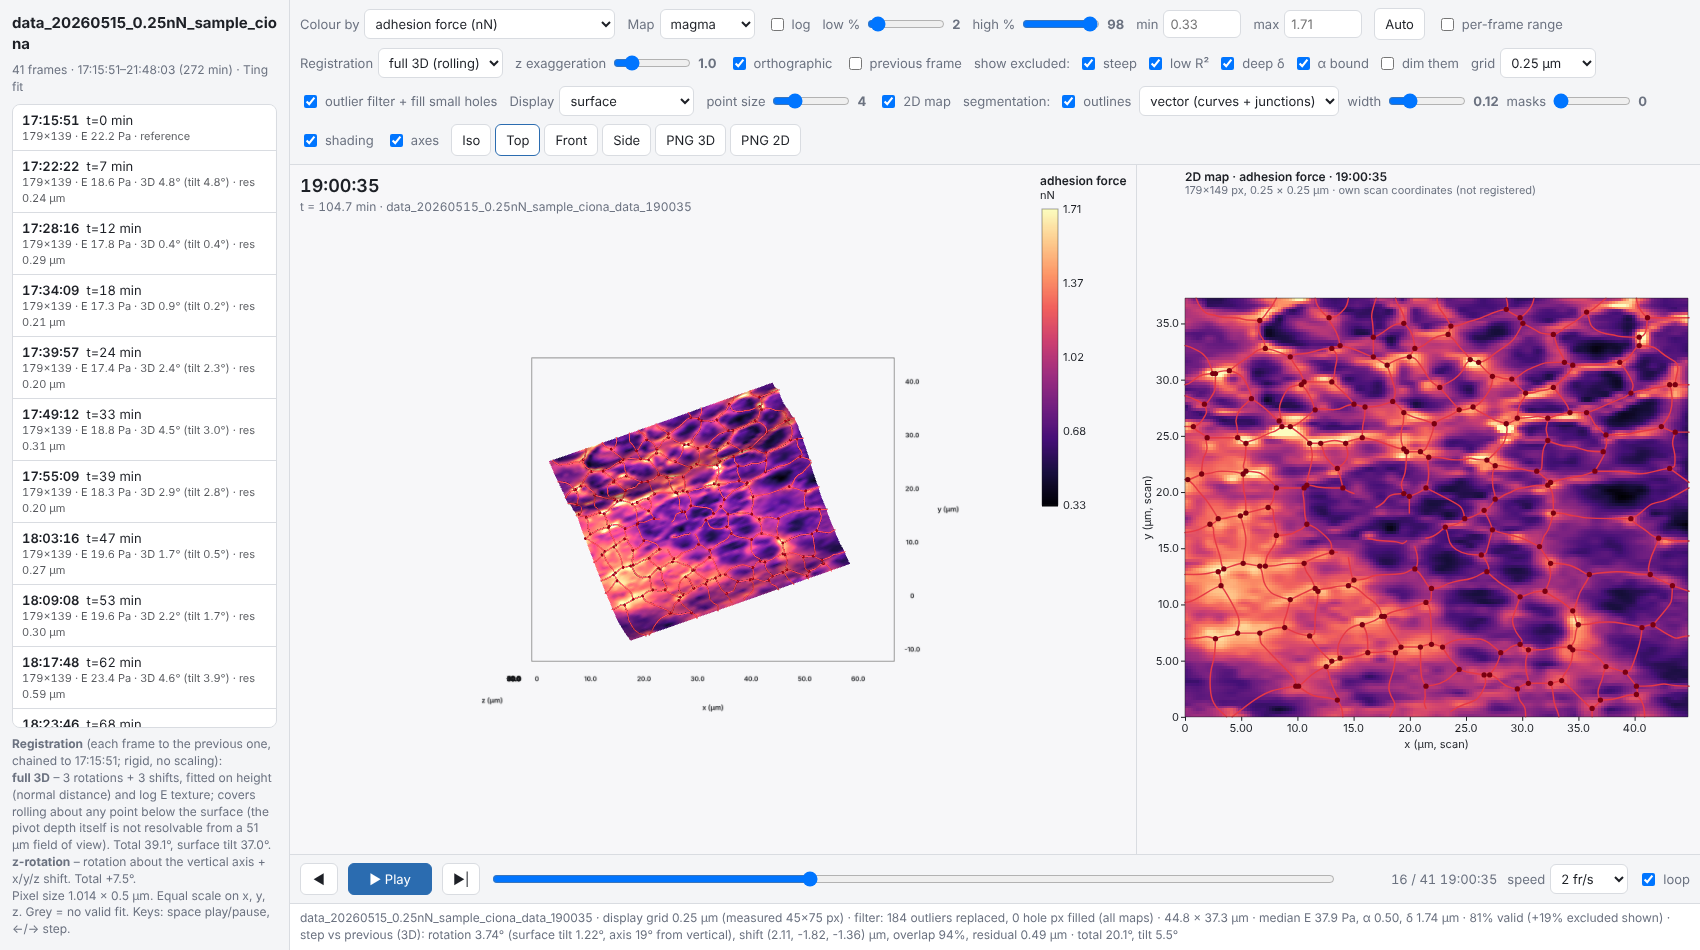
\includegraphics[width=\textwidth]{fig/viewer.png}
\end{column}
\begin{column}{0.4\textwidth}
\begin{lstlisting}
python build_timelapse_viewer.py maps -o viewer.html --config afm_pipeline.toml
\end{lstlisting}
\footnotesize
\begin{itemize}
\item One HTML file with all data embedded (no internet needed). Open it in any browser.
\item The frames are registered in 3D (rigid). Registration modes: full 3D, $z$-rotation, or raw.
\item Controls:
 \begin{itemize}
 \item colour by any map; colour range;
 \item excluded pixels per reason, and \emph{dim them};
 \item display grid and outlier filter;
 \item surface or points;
 \item cell outlines (vector or pixels) and masks;
 \item linked 2D map; play / step / loop; PNG export.
 \end{itemize}
\item Keys: space = play, $\leftarrow/\rightarrow$ = step.
\end{itemize}
\end{column}
\end{columns}
\end{frame}

\begin{frame}[fragile]{A complete session}
\begin{lstlisting}
# 0. once: copy the template and set calibration + probe
cp afm_pipeline.toml my_experiment.toml   # then edit [afm], [probe], cell_diameter_um

# 1. fit every map below the raw-data root
python afm_ting_pipeline.py /data/data_20260515_0.25nN -o results --config my_experiment.toml

# 2. export maps (+ pixels.json, excluded/)
python extract_topo_E.py results -o maps --config my_experiment.toml

# 3. segment and track cells (time-lapse only)
python segment_cells.py maps -o seg --config my_experiment.toml

# 4. viewer
python build_timelapse_viewer.py maps -o viewer.html --config my_experiment.toml
\end{lstlisting}
\small
On Windows use \texttt{py} instead of \texttt{python}, \texttt{copy} instead of \texttt{cp}, and paths like \texttt{D:\textbackslash data\textbackslash ...}. Paths with spaces need quotes.\\[3pt]
Steps 2--4 take seconds to minutes and can be repeated with other parameters at any time. Only step 1 refits the curves.
\end{frame}

% ===========================================================================
\section{Checks and troubleshooting}

\begin{frame}{Troubleshooting}
\footnotesize
\begin{tabularx}{\textwidth}{@{}>{\raggedright\arraybackslash}p{0.32\textwidth} X@{}}
\toprule
message / symptom & cause and fix\\
\midrule
\texttt{no datasets found} & the folder has no \texttt{config.txt} next to \texttt{ForceCurve\_*.lvm}; check the structure, or give the data-set folders directly\\
\texttt{[warn] N files but grid is ...} & missing or extra \texttt{.lvm} files; missing pixels become empty\\
\texttt{[config] unknown key ...} & typo in the config file (the key is ignored)\\
\texttt{[skip] ... exists} & result already there; use \texttt{--overwrite}\\
very low valid fraction, $R^2<0.9$ & wrong InvOLS, $k$ or $Z$ sensitivity; trigger force too low; probe geometry wrong\\
$E$ off by a constant factor & calibration ($k$, InvOLS) or $R$; the relative maps stay correct\\
striped or shifted maps & \texttt{zigzag} wrong (\texttt{[acquisition] zigzag = true/false})\\
\texttt{no pixels.json ... assuming ...} & maps exported with an old \texttt{extract\_topo\_E.py}: rerun step 2, or give \texttt{--px --py}\\
registration: large rotation, low overlap & frames do not overlap enough, or a frame was aborted; check that frame; \texttt{[registration] recompute = true} after changes\\
segmentation: cells split / merged & \texttt{seed\_depth} up / down, or set \texttt{cell\_diameter\_um}\\
viewer: grey pixels & excluded or no data; tick the reasons under \emph{show excluded}\\
\bottomrule
\end{tabularx}
\end{frame}

\begin{frame}{Checklist for a new data set}
\small
\begin{enumerate}
\item The folder structure is as on the input-data slide. Map folders end in HHMMSS for time-lapses.
\item \texttt{[afm]} and \texttt{[probe]} are set for this cantilever and probe.
\item Run step 1 on one map first. Check:
 \begin{itemize}
 \item the speeds and drag in the log;
 \item valid fraction $>90\,\%$ and median $R^2\approx0.95$--0.99;
 \item the quick-look PNG: is the topography plausible, and are the maps without stripes?
 \end{itemize}
\item Run all maps, then step 2. Check \texttt{pixels.json} against the scan size and grid.
\item Time-lapse: build the viewer and check the registration (residuals and overlap in the log; play the sequence).
\item Set \texttt{cell\_diameter\_um} from the maps (count cells along a line), run step 3, and check \texttt{segmentation\_overview.png}.
\item Archive the config file together with the results (it is also stored inside every \texttt{.npz}).
\end{enumerate}
\vspace{4pt}
\textbf{Further documentation} (in \texttt{docs/}):
\begin{itemize}
\item \texttt{ting/}: the Ting fit;
\item \texttt{adhesion/}: the adhesion properties;
\item \texttt{segmentation/}: segmentation and tracking.
\end{itemize}
\end{frame}

\end{document}
